\section{Wellen}
\begin{itemize}
    \setlength\itemsep{1pt}
    \item Ausbreitungsphänomen von E und H
    \item Ausbreitungsgeschw. kleiner $c_0$
    \item raumzeitlicher Vorgang $cos(\omega t- \beta z)$
    \item Energie- ohne Materietransport
    \item Poyntingvektor $\vec{S}=\vec{E}\times\vec{H}$ Einheit[S]$= \dfrac{W}{m^2}$\\
          {\footnotesize Falls $\vec{E}\perp\vec{H}$ und $\vec{S}\perp\vec{E}$ und $\vec{S}\perp\vec{H}$}
\end{itemize}

\subsubsection*{Wellengleichung}
\makebox[0pt][l]{
    \begin{minipage}{\columnwidth}
        \centering
        \[
            \boxed{\vec{E} = \underbrace{E_0}_{\mathclap{\text{Amplitude}}}
            \cdot \overbrace{e^{-\alpha z}}^{\mathclap{\text{Dämpfung}}}
            \cdot \underbrace{cos(\omega t \overbrace{-}^{\mathclap{\text{positive z-Richtung}}} \beta z)}_\text{Zeit- und Raumabhängigkeit}}
        \]
        {\footnotesize Analog für H-Feld}
    \end{minipage}
}

\subsubsection*{Fortpflanzungskonstante $\gamma$}
\[\boxed{\underline{\gamma}=\alpha+j\beta}\]

$\alpha$ : Dämpfungskonstante [Np/m]

$\beta$ : Phasenkonstante [rad/m]

$v$ : Phasengeschwindigkeit [m/s]

\subsection{Ausbreitung}
\subsubsection{Allgemein}
\begin{align*}
    \lambda                 & = \dfrac{2\pi}{\beta} \qquad E_2 = E_1 e^{-\alpha z}                                                                                        \\
    v_{ph}                  & = \lambda\cdot f                                                                                                                            \\
    \alpha                  & = \omega \cdot \sqrt{\dfrac{\mu \varepsilon}{2}\cdot \left(\sqrt{1+\dfrac{\sigma^2}{\omega^2\cdot\varepsilon^2}}{\color{red}{-}}1\right)}   \\
    \beta                   & = \omega \cdot \sqrt{\dfrac{\mu \varepsilon}{2}\cdot \left(\sqrt{1+\dfrac{\sigma^2}{\omega^2\cdot\varepsilon^2}}{\color{green}{+}}1\right)} \\
    \Aboxed{\underline{Z}_F & = \dfrac{\underline{E}_\text{transversal}}{\underline{H}_\text{transversal}} = \sqrt{\dfrac{j\omega\mu}{\sigma+j\omega\varepsilon}}}        \\
\end{align*}

\subsubsection{Im leeren Raum(Vakuum)}
\begin{align*}
    \alpha                     & = 0                                                    \\
    \beta                      & = \dfrac{\omega}{c_0}                                  \\
    \lambda                    & = \dfrac{c_0}{f}                                       \\
    v                          & = c_0                                                  \\
    \Aboxed{\underline{Z}_{F0} & = \sqrt{\dfrac{\mu_0}{\varepsilon_0}}\approx377\Omega}
\end{align*}

\subsubsection{Im verlustlosen/idealen Dielektrika}
verlustlos: $\sigma =0$, maximale Wirkleistung

$Z_F$ rein reel $\rightarrow$ ebene Welle
\begin{align*}
    \alpha                  & = 0                                                                                              \\
    \beta                   & = \dfrac{\omega}{c_0}\sqrt{\mu_r\varepsilon_r}=\omega\sqrt{\mu\varepsilon}=\dfrac{2\pi}{\lambda} \\
    \lambda                 & = \dfrac{c_0}{f}\dfrac{1}{\sqrt{\mu_r\varepsilon_r}}                                             \\
    v                       & = \dfrac{c_0}{\sqrt{\mu_r\varepsilon_r}}                                                         \\
    \Aboxed{\underline{Z}_F & = \sqrt{\dfrac{\mu}{\varepsilon}}}
\end{align*}

\subsubsection{Im Dielektrika mit geringem Verlust}
geringer Verlust: $0 < \sigma \ll\omega\varepsilon$

\begin{align*}
    \alpha                  & = \dfrac{\sigma}{2}\cdot\sqrt{\dfrac{\mu}{\varepsilon}} = \frac{\sigma}{2}\cdot Z_{F0}               \\
    \beta                   & = \omega\sqrt{\mu\varepsilon}\left(1+\dfrac{1}{8}\cdot\dfrac{\sigma^2}{\omega^2\varepsilon^2}\right) \\
    \lambda                 & = \dfrac{c_0}{f}\cdot\dfrac{1}{\sqrt{\mu_r\varepsilon_r}}                                            \\
    v                       & = \dfrac{c_0}{\sqrt{\mu_r\varepsilon_r}}                                                             \\
    \Aboxed{\underline{Z}_F & = \sqrt{\dfrac{\mu}{\varepsilon}}}
\end{align*}

\subsubsection{Im guten Leiter}
geringer Verlust: $\sigma \gg\omega\varepsilon$
\begin{align*}
    \alpha                  & = \beta = \dfrac{1}{\delta} \sim \sqrt{f}                             \\
    \lambda                 & = 2\pi \sqrt{\dfrac{2}{\omega\mu\sigma}}=2\pi\delta                   \\
    \Aboxed{\underline{Z}_F & = \sqrt{\dfrac{j\omega\mu}{\sigma}} = \dfrac{1+j}{\sigma\cdot\delta}}
\end{align*}

\subsection{Übergang}
\subsubsection{Zwischen Dielektrika mit geringem Verlust}

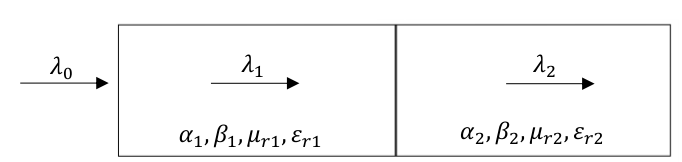
\includegraphics[width=\columnwidth]{Figures/UebergangzweiDielektrika.png}
\begin{align*}
    \quad \qquad \lambda_1 & = \dfrac{\lambda_0}{\sqrt{\mu_{r1}\varepsilon_{r1}}}          & \lambda_2 & = \dfrac{\lambda_0}{\sqrt{\mu_{r2}\varepsilon_{r2}}}                                     \\
    \quad \qquad           &                                                               &           & = \dfrac{\lambda_1\cdot\sqrt{\mu_{r1}\varepsilon_{r1}}}{\sqrt{\mu_{r2}\varepsilon_{r2}}} \\
    \quad \qquad \beta_1   & = \dfrac{2\pi}{\lambda_0}\cdot\sqrt{\mu_{r1}\varepsilon_{r1}} & \beta_2   & = \dfrac{2\pi}{\lambda_0}\cdot\sqrt{\mu_{r2}\varepsilon_{r2}}                            \\
    \quad \qquad Z_{F1}    & = \dfrac{Z_{F0}}{\sqrt{\mu_{r1}\varepsilon_{r1}}}             & Z_{F2}    & = \dfrac{Z_{F0}}{\sqrt{\mu_{r2}\varepsilon_{r2}}}
\end{align*}

\subsection{Energie und Poyntingvektor (Energieflussdichte)}
\begin{align*}
     & \vec{S} = \vec{E}\times\vec{H} \text{ in } [W/m^2]                                   \\
     & S = 1/2 \cdot E \cdot H = 1/2 \cdot \dfrac{E^2}{Z_{F0}} = 1/2 \cdot H^2 \cdot Z_{F0} \\
     & \underline{S}_{\texttt{Mittel}} = 1/2 \cdot Re\{\vec{E}\times\vec{H}^*\}             \\
     & S = \dfrac{P}{A}                                                                     \\
\end{align*}

\subsubsection{Leistung nach Dämpfung}
\begin{align*}
     & P_1 = P_0 \cdot e^{-2\alpha z}                              \\
     & P = \dfrac{\hat{U}^2}{2 Z_L} \text{vom Kabel transportiert}
\end{align*}

\subsection{dÀlembertsche Gleichung (allg.)}
\begin{align*}
    \Delta \vec{E}-\kappa \mu \frac{\partial \vec{E}}{\partial t}-\varepsilon \mu \frac{\partial^{2} \vec{E}}{\partial t^{2}} & = \operatorname{grad} \frac{\rho}{\varepsilon} \\
    \Delta \vec{H}-\kappa \mu \frac{\partial \vec{H}}{\partial t}-\varepsilon \mu \frac{\partial^{2} \vec{H}}{\partial t^{2}} & = 0
\end{align*}

Isolator, ideales Dielektrikum, Nichtleiter $\kappa = 0$
\begin{align*}
    \Delta \vec{E} & =\varepsilon \mu \frac{\partial^{2} \vec{E}}{\partial t^{2}}+\operatorname{grad} \frac{\rho}{\varepsilon} \\
    \Delta \vec{H} & =\varepsilon \mu \frac{\partial^{2} \vec{H}}{\partial t^{2}}
\end{align*}

sehr gute Leiter
\begin{align*}
    \Delta \vec{E} & =\kappa \mu \frac{\partial \vec{E}}{\partial t}+\operatorname{grad} \frac{\rho}{\varepsilon} \\
    \Delta \vec{H} & =\kappa \mu \frac{\partial \vec{H}}{\partial t}
\end{align*}

\subsection{Helmholtz-Gleichungen (Frequenzbereich)}
\begin{align*}
    \Delta \underline{\vec{E}}-\left(\kappa \mu \cdot \mathrm{j} \omega-\varepsilon \mu \cdot \omega^{2}\right) \cdot \underline{\vec{E}} & = \operatorname{grad} \frac{\rho}{\varepsilon} \\
    \Delta \underline{\vec{H}}-\left(\kappa \mu \cdot \mathrm{j} \omega-\varepsilon \mu \cdot \omega^{2}\right) \cdot \underline{\vec{H}} & = 0
\end{align*}

\subsubsection{Zeitbereich}
\begin{align*}
    \Delta \vec{E}-\varepsilon \mu \frac{\partial^{2} \vec{E}}{\partial t^{2}} & =0 \\
    \Delta \vec{H}-\varepsilon \mu \frac{\partial^{2} \vec{H}}{\partial t^{2}} & =0
\end{align*}

\subsubsection{Frequenzbereich (harmonisch)}
\begin{align*}
    \Delta \underline{\vec{E}}+\varepsilon \mu \omega^{2} \cdot \underline{\vec{E}} & =0 \\
    \Delta \underline{\vec{H}}+\varepsilon \mu \omega^{2} \cdot \underline{\vec{H}} & =0
\end{align*}

%%%%%%%%%%%%%%%%%

\subsection{Wellenzahl}
Im Vakuum: $k_{0}=\frac{\omega}{c_{0}}$
\begin{align*}
    k & = \frac{\omega}{v_{p h}} = \frac{2 \pi f}{v_{p h}} = |\vec{k}|                                                              \\
      & = \frac{\omega \cdot n}{c_{0}} = n \cdot k_{0}=\frac{1}{\sqrt{\mu_{r} \cdot \varepsilon_{r}}} \cdot k_{0}=k_{r} \cdot k_{0}
\end{align*}

\subsection{Wellenlänge}
\begin{align*}
    \lambda   & = \dfrac{\lambda_0}{\sqrt{\mu_r \cdot \varepsilon_r}} = \dfrac{2 \pi}{k} = \dfrac{v_{ph}}{f} = [m] \\
              & = \dfrac{\lambda_0}{n} = \dfrac{2 \pi}{n \cdot k_0}                                                \\
    \lambda_0 & = \dfrac{c_0}{f} = \dfrac{2\pi}{k_0}
\end{align*}

\subsection{Phasengeschwindigkeit}
\[
    \dfrac{d z}{d t} = \upsilon_{ph} = c = \dfrac{\omega}{k} = \frac{1}{\sqrt{ \mu_r \mu_0 \varepsilon_r \varepsilon_0}} \qquad \upsilon_{ph,\texttt{Medium} \leq c_0}
\]

\subsubsection{Gruppengeschwindigkeit}
\[
    \upsilon_{g} = \dfrac{d \omega}{d k} = \dfrac{\textnormal{Wegstück der Wellengruppe}}{\textnormal{Laufzeit der Wellengruppe}}
\]

\subsection{Polarisation}
\begin{tabularx}{0.45\textwidth}{>{\hsize=.27\hsize}X|>{\hsize=.5\hsize}X|>{\hsize=.23\hsize}X}
    Lineare      & wenn der Endpunkt des E–Vektors eine Linie beschreibt & $H$ oder $E$ \\
    \hline
    Elliptische  & Endpunkt des E-Vektors eine Ellipse beschreibt        & $E\neq H$    \\
    \hline
    Kreisförmige & der Endpunkt des E-Vektors einen Kreis beschreibt     & $E = H$      \\
\end{tabularx}

\subsubsection{Senkrechte Polarisation}

\begin{tikzpicture}
    \draw[dotted] (-3,0) -- (3,0);
    \draw[-] (0,-4) -- (0,4)                node[below right] {$\varepsilon_{r2}, \mu_{r2}, \sigma_{r2}$}
                                            node[below left] {$\varepsilon_{r1}, \mu_{r1}, \sigma_{r1}$};

    \draw[->] (-3,3) -- (-1.5,1.5)          node[above right] {$S_h$};
    \draw[->] (-3,3) -- (-3.5,2.5)          node[below right] {$H_h$};
    \draw[-] (-3,3) circle (0.15)           node[above] {$E_h$};
    \draw[dotted] (-3,3) -- (0,0);
    \draw[<->] (135:0.5) arc (135:180:0.5); 
    \node[] at (-0.8,0.2) {$\alpha$};

    \draw[->] (-1.5,-1.5) -- (-2,-2)        node[above left] {$S_r$};
    \draw[->] (-1.5,-1.5) -- (-1.8,-1.2)    node[above] {$H_r$};
    \draw[-] (-1.5,-1.5) circle (0.15)      node[right] {$E_r$};
    \draw[dotted] (-3,-3) -- (0,0);
    \draw[<->] (180:0.5) arc (180:225:0.5);
    \node[] at (-0.8,-0.2) {$\alpha$};

    \draw[->] (2,-0.6666) -- (3,-1)         node[above right] {$S_g$};
    \draw[->] (2,-0.6666) -- (1.3333,-2.8)  node[below right] {$H_g$};
    \draw[-] (2,-0.6666) circle (0.15)      node[above] {$E_g$};
    \draw[dotted] (0,0) -- (3,-1);
    \draw[<->] (0:1) arc (0:-20:1);     
    \node[] at (1.3,-0.2) {$\beta$};

\end{tikzpicture}

\begin{itemize}
    \item mag./elek. Reflexionsfaktor $[1]$
    \item mag. Transmissionsfaktor $[1]$
    \item elek. Transmissionsfaktor $[1]$
\end{itemize}

\begin{align*}
    r_{m s} & = \frac{Z_{F 2} \cdot \cos \alpha-Z_{F 1} \cdot \cos \beta}{Z_{F 2} \cdot \cos \alpha+Z_{F 1} \cdot \cos \beta} = r_{e s} = r_{s} \\
    t_{m s} & = \frac{2 \cdot Z_{F 1} \cdot \cos \alpha}{Z_{F 2} \cdot \cos \alpha+Z_{F 1} \cdot \cos \beta}                                    \\
    t_{e s} & = \frac{2 \cdot Z_{F 2} \cdot \cos \alpha}{Z_{F 2} \cdot \cos \alpha+Z_{F 1} \cdot \cos \beta}                                    \\
    t_{e s} & -r_{e s}= 1 \qquad t_{m s} = (1 - r_{m s}) \cdot \dfrac{\cos \alpha}{\cos \beta}                                                  \\
    E_{g}   & = t_{e s} \cdot E_{h} \qquad E_{r} = r_{s} \cdot E_{h}                                                                            \\
    H_{g}   & = t_{m s} \cdot H_{h} \qquad H_{r} = r_{s} \cdot H_{h}
\end{align*}

\subsubsection{Parallel Polarisation}
\begin{tikzpicture}
    \draw[dotted] (-3,0) -- (3,0);
    \draw[-] (0,-4) -- (0,4)                node[below right] {$\varepsilon_{r2}, \mu_{r2}, \sigma_{r2}$}
                                            node[below left] {$\varepsilon_{r1}, \mu_{r1}, \sigma_{r1}$};

    \draw[->] (-3,3) -- (-1.5,1.5)          node[above right] {$S_h$};
    \draw[->] (-3,3) -- (-3.5,2.5)          node[below right] {$E_h$};
    \draw[-] (-3,3) circle (0.15)           node[above] {$H_h$};
    \draw[dotted] (-3,3) -- (0,0);
    \draw[<->] (135:0.5) arc (135:180:0.5); 
    \node[] at (-0.8,0.2) {$\theta_h$};

    \draw[->] (-1.5,-1.5) -- (-2,-2)        node[above left] {$S_r$};
    \draw[->] (-1.5,-1.5) -- (-1.8,-1.2)    node[above] {$E_r$};
    \draw[-] (-1.5,-1.5) circle (0.15)      node[right] {$H_r$};
    \draw[dotted] (-3,-3) -- (0,0);
    \draw[<->] (180:0.5) arc (180:225:0.5);
    \node[] at (-0.8,-0.2) {$\theta_r$};

    \draw[->] (2,-0.6666) -- (3,-1)         node[above right] {$S_t$};
    \draw[->] (2,-0.6666) -- (1.3333,-2.8)  node[below right] {$E_t$};
    \draw[-] (2,-0.6666) circle (0.15)      node[above] {$H_t$};
    \draw[dotted] (0,0) -- (3,-1);
    \draw[<->] (0:1) arc (0:-20:1);     
    \node[] at (1.3,-0.2) {$\theta_t$};

\end{tikzpicture}

\begin{itemize}
    \item mag./elek. Reflexionsfaktor $[1]$
    \item mag. Transmissionsfaktor $[1]$
    \item elek. Transmissionsfaktor $[1]$
\end{itemize}

\begin{align*}
    r_{m p} & = \frac{Z_{F 1} \cos \vartheta_{1}-Z_{F 2} \cos \vartheta_{2}}{Z_{F 1} \cos \vartheta_{1}+Z_{F 2} \cos \vartheta_{2}} = r_{e p} = \frac{E_{r 0}}{E_{h 0}} =r_{p} \\
    t_{m p} & = \frac{2 Z_{F 1} \cos \vartheta_{1}}{Z_{F 1} \cos \vartheta_{1}+Z_{F 2} \cos \vartheta_{2}}                                                                     \\
    t_{e p} & = \frac{2 Z_{F 2} \cos \vartheta_{1}}{Z_{F 1} \cos \vartheta_{1}+Z_{F 2} \cos \vartheta_{2}} = \frac{Z_{F 2}}{Z_{F 1}} t_{m p}
\end{align*}
